\chapter{Grundlagen und Verwandte Arbeiten}\label{sec:basics}

% In diesem Kapitel landet alles,
% was nicht vom Autor selbst erfunden wurde.
% Einerseits Grundlagen,
% die für das Verständnis der Arbeit notwendig sind.
% Andererseits verwandte Arbeiten,
% wobei bei diesen klar gemacht werden soll,
% inwiefern diese Arbeit darauf aufbaut bzw. etwas anders macht.

% Beispiel wäre ein Standardwerk in Sachen SSA-Form~\cite{cytron91}
% welches bei uns häufig zitiert wird.

% Es soll klar werden,
% dass dem Studenten der Stand der Technik bewusst war
% und keine redundante Arbeit gemacht wurde.

% Compiler
\section{Compiler}\label{sec:basics:compiler}

The basic function of a compiler is to automatically convert high-level code created by a developer into (optimized) machine code.
As a compiler is an inherently large software project, the architecture needs to be chosen that allows for extensions and modifications easily.
Modern compilers mostly follow a layered architecture style: They each entice a front-, middle-, and back-end.
In this architecture, the front-end will convert the high-level code into an abstract intermediary representation that is then used by the middle-end for optimizations and transformations.
Lastly, the backend is responsible for converting the optimized intermediary code into instructions for the target system (e.g. \texttt{RISC-V}, \texttt{x86}, \texttt{ARM}, etc.)

% Basic blocks
\section{Basic blocks and control-flow}\label{sec:basics:bb-cf}

Most compilers will divide code up into so-called \textit{basic blocks}.
Basic blocks are sets of consecutive operations that do not contain jumps within them, but rather only jumps connecting them.
Henceforth, a basic block will either be executed completely or not executed at all.

A usual way to represent this in a human-readable form is to output it as a control-flow-graph (CFG).
In a CFG a basic block is depicted as a node and jumps between basic blocks are represented by edges.
Further, it is a convention in these graphs to have exactly one start and one end node.

It is to be noted that CFGs, in general, are cyclical graphs.
They merely are non-cyclical graphs, iff the original code does not contain any jumps going backward in the control-flow.

Another important concept of CFGs is dominance.
In order to explain this concept, a starting node $S$ is defined and assume we have any two nodes from the CFG $N_1$, and $N_2$.
$$N_1~\text{dominates}~N_2 \Longleftrightarrow \forall p \in \text{Paths}(S, N_2),~N_1 \in p$$
In plain english this means that $N_1$ dominates $N_2$, iff in order to get to $N_2$ from $S$ you have to visit $N_1$ on the way.
Please also note that a block always dominates itself.

% Lifetime

\section{Loops}\label{sec:basics:loops}

A loop has been defined as a set of nodes that are all in a cyclical control-flow structure.
Loops can furthermore have a header, which is the sole entry point into a loop~\cite{aebi18bachelorarbeit} and defined as follows

$$N~\text{is header of}~L \Longleftrightarrow N \in L \wedge \forall n \in L: N~\text{dominates}~n$$

N.B.: Not all loops have to have a header.

% SSA
\section{Single-Static-Assignment (SSA)}\label{sec:basics:ssa}

The \textit{single-static-assignment} (\textit{SSA}) form is a property of intermediary representations, that requires each variable to only be assigned exactly once.
Moreover, every variable has to be assigned before it is being used~\cite{cytron91}.
This especially implies that the block in which a given variable $v$ is declared has to dominate all blocks in which $v$ is used.
An example of a program in SSA form can be seen in~\cref{fig:basics:SSA-simple}.

\begin{figure}[h]
    \begin{minipage}[t]{0.5\textwidth}
        \centering
        \begin{algorithmic}
            \State $x \gets 1$
            \State \Call{Print}{$x$}
            \State $x \gets 7$
            \State \Call{Print}{$x$}
        \end{algorithmic}
        Base code
    \end{minipage}
    \begin{minipage}[t]{0.5\textwidth}
        \centering
        \begin{algorithmic}
            \State $x_1 \gets 1$
            \State \Call{Print}{$x_1$}
            \State $x_2 \gets 7$
            \State \Call{Print}{$x_2$}
        \end{algorithmic}
        Code in SSA form
    \end{minipage}
    \caption{An example program in SSA form}
    \label{fig:basics:SSA-simple}
\end{figure}

In a loop or a conditional statement, a scenario might arise where multiple values could be assigned to a given variable.
In cases like these a $\Phi$-function can be used.
A $\Phi$-function is a theoretical construct that will return the correct value depending on the control-flow predecessor.

An example the use of a $\Phi$-function this can be seen in~\cref{fig:basics:SSA-phi}, where a depending on the control-flow either $m_1$ or $m_2$ are selected.

\begin{figure}[h]
    \begin{minipage}[t]{0.5\textwidth}
        \centering
        \begin{algorithmic}
            \Function{max}{$a: \mathbb{N},b: \mathbb{N}$}
                \State $m: \mathbb{N}$
                \If{a > b}
                    \State $m \gets a$
                \Else
                    \State $m \gets b$
                \EndIf
                \State \Return $m$
            \EndFunction
        \end{algorithmic}
        Code in SSA form
    \end{minipage}
    \begin{minipage}[t]{0.5\textwidth}
        \centering
        \begin{algorithmic}
            \Function{max}{$a: \mathbb{N},b: \mathbb{N}$}
                \State $m: \mathbb{N}$
                \If{$a > b$}
                    \State $m_1 \gets a$
                \Else
                    \State $m_2 \gets b$
                \EndIf
                \State $m \gets$ \Call{$\Phi$}{$m_1, m_2$}
                \State \Return m
            \EndFunction
        \end{algorithmic}
        Base code
    \end{minipage}
    \caption{An example program in SSA form}
    \label{fig:basics:SSA-phi}
\end{figure}

% LCSAA

\section{Loop-Closed-Single-Static-Assignment (LCSSA)}\label{sec:basics:LCSSA}

An extension to the SSA form is the \textit{loop-closed-single-static-assignment} (\textit{LCSSA}) form.
It in addition to the properties guaranteed by the regular SSA form a CFG in LCSSA has the property that each variable that lives across a loop boundary is required to have a phi node in the first block after a loop~\cite{LLVM_LCSSA}.
To visualize this property,~\cref{fig:basics:LCSSA} depicts its effect.

\begin{figure}[h]
    \begin{minipage}[t]{0.5\textwidth}
        \centering
        \begin{algorithmic}
            \Function{Foo}{}
            \State $x, y: \mathbb{N}$
            \Repeat
            \If{\Call{Condition}{}}
            \State $x_1 \gets 5$
            \Else
            \State $x_2 \gets 8$
            \EndIf
            \State $x \gets \Phi(x_1, x_2)$
            \Until{\Call{OtherCondition}{}}
            \State $y \gets x + 3$
            \EndFunction
        \end{algorithmic}
        Code in SSA form
    \end{minipage}
    \begin{minipage}[t]{0.5\textwidth}
        \centering
        \begin{algorithmic}
            \Function{Foo}{}
            \State $x, y: \mathbb{N}$
            \Repeat
            \If{\Call{Condition}{}}
            \State $x_1 \gets 5$
            \Else
            \State $x_2 \gets 8$
            \EndIf
            \State $x_3 \gets \Phi(x_1, x_2)$
            \Until{\Call{OtherCondition}{}}
            \State $x \gets \Phi(x_3)$
            \State $y \gets x + 3$
            \EndFunction
        \end{algorithmic}
        Code in LCSSA form
    \end{minipage}
    \caption{An example program transformed into LCSSA Form (adapted from~\cite{LLVM_LCSSA})}
    \label{fig:basics:LCSSA}
\end{figure}


% FIRM
\section{\libFIRM}\label{sec:basics:firm}

\libFIRM~is a compiler middle- and back-end that takes a graph-based intermediate representation in SSA form, optimizes it and produces assembly code~\cite{libfirm}.
Since 1996 \libFIRM~is developed at Karlsruhe Institute of Technology (KIT).

A graph in \libFIRM~contains information about basics blocks, the control-flow, memory and, data dependencies.
Basics blocks in \libFIRM~contain further nodes that are responsible for the control-flow of the program.
These are pointed to by (other) basic blocks that are the target of these control-flow operations.
The resulting control-flow edges will be represented by a red edge in visualizations of \libFIRM~graphs.
Any node that does an operation on memory will be connected to memory nodes that are responsible for always assuring the current state of memory.
Memory is, like control flow, connected by edges, which are rather than being colored red blue in graphical representations.
Lastly, \libFIRM~has data dependency edges between nodes, which represent dependencies needed for calculations.

In~\cref{fig:basics:firm} we can see an example firm graph of the program originally shown in~\cref{fig:basics:SSA-phi}.
It is especially to be noted that the graph is in SSA form, as it contains the phi node and has both memory, data and, control-flow edges.

\begin{figure}
    \centering
    % Scale factor 0.04065040650406504
\definecolor{color10}{RGB}{204,204,204}
\definecolor{color11}{RGB}{222,239,234}
\definecolor{color12}{RGB}{255,153,255}
\definecolor{color13}{RGB}{255,153,153}
\definecolor{color14}{RGB}{153,255,153}
\definecolor{color15}{RGB}{0,150,60}
\definecolor{color16}{RGB}{153,153,255}
\definecolor{color17}{RGB}{255,255,255}
\definecolor{color18}{RGB}{255,0,0}
\definecolor{color19}{RGB}{0,0,0}
\definecolor{color20}{RGB}{100,100,255}
% Bounding Box: 369.0, 862.0
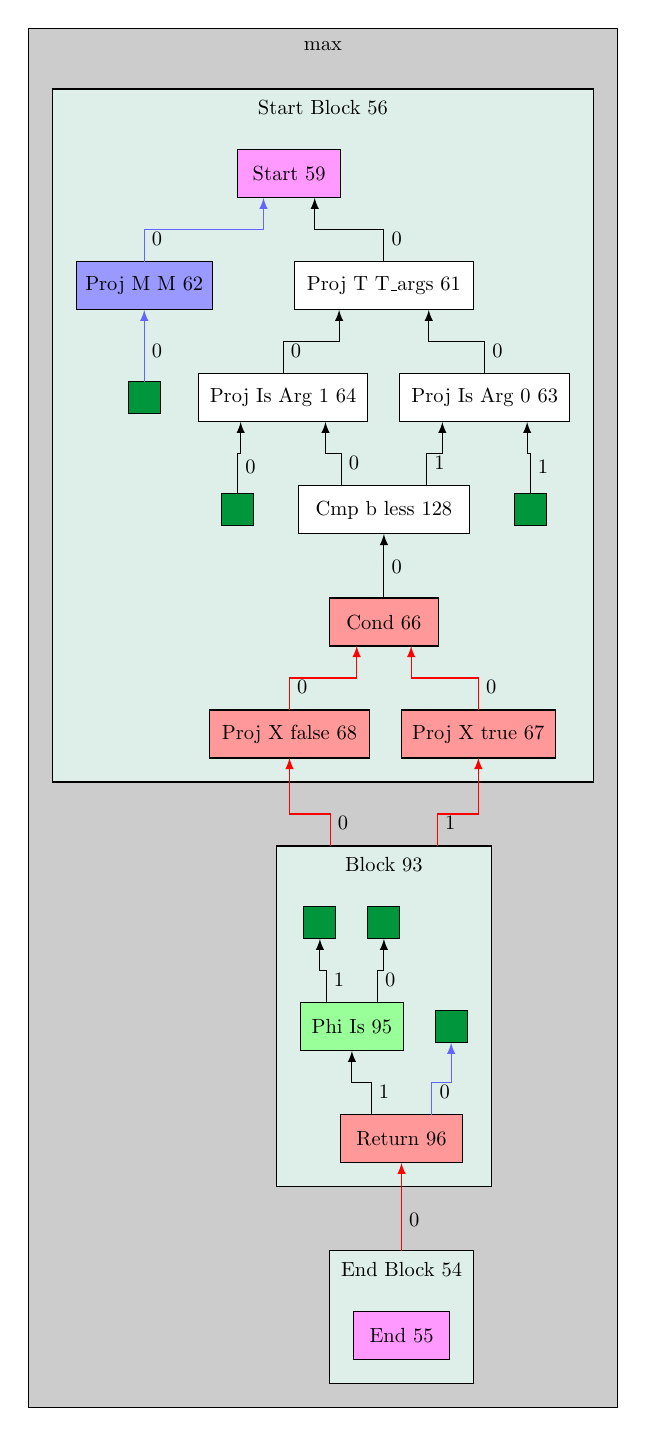
\begin{tikzpicture}[scale=0.5, transform shape]
	\node[fill=color10, draw, minimum width=14.96951219512195cm, minimum height=35.040650406504064cm] (n26) at (7.484756097560975cm ,17.520325203252032cm) {};
	% 1 node layouts
	\node[scale=1.4781966001478197, transform shape] at (7.484756097560975cm ,34.57634654471545cm) {max};
	\node[fill=color11, draw, minimum width=13.75cm, minimum height=17.601626016260163cm] (n27) at (7.484756097560975cm ,24.695121951219512cm) {};
	% 1 node layouts
	\node[scale=1.4781966001478197, transform shape] at (7.484756097560975cm ,33.031631097560975cm) {Start Block  56};
	\node[fill=color11, draw, minimum width=5.447154471544716cm, minimum height=8.658536585365853cm] (n28) at (9.034552845528456cm ,9.939024390243903cm) {};
	% 1 node layouts
	\node[scale=1.4781966001478197, transform shape] at (9.034552845528456cm ,13.80398882113821cm) {Block  93};
	\node[fill=color11, draw, minimum width=3.6585365853658547cm, minimum height=3.3739837398373984cm] (n29) at (9.481707317073171cm ,2.296747967479675cm) {};
	% 1 node layouts
	\node[scale=1.4781966001478197, transform shape] at (9.481707317073171cm ,3.519435975609756cm) {End Block  54};
	\node[fill=color12, draw, minimum width=2.4390243902439024cm, minimum height=1.2195121951219512cm] (n30) at (9.48170731707317cm ,1.8292682926829267cm) {};
	% 1 node layouts
	\node[scale=1.4781966001478197, transform shape] at (9.48170731707317cm ,1.8292682926829267cm) {End  55};
	\node[fill=color13, draw, minimum width=3.089430894308943cm, minimum height=1.2195121951219512cm] (n31) at (9.48170731707317cm ,6.829268292682927cm) {};
	% 1 node layouts
	\node[scale=1.4781966001478197, transform shape] at (9.48170731707317cm ,6.829268292682927cm) {Return  96};
	\node[fill=color14, draw, minimum width=2.6016260162601625cm, minimum height=1.2195121951219512cm] (n32) at (8.221544715447154cm ,9.674796747967479cm) {};
	% 1 node layouts
	\node[scale=1.4781966001478197, transform shape] at (8.221544715447154cm ,9.674796747967479cm) {Phi Is 95};
	\node[fill=color15, draw, minimum width=0.8130081300813008cm, minimum height=0.8130081300813008cm] (n33) at (10.741869918699187cm ,9.674796747967479cm) {};
	\node[fill=color15, draw, minimum width=0.8130081300813008cm, minimum height=0.8130081300813008cm] (n34) at (9.034552845528454cm ,12.317073170731707cm) {};
	\node[fill=color15, draw, minimum width=0.8130081300813008cm, minimum height=0.8130081300813008cm] (n35) at (7.4085365853658525cm ,12.317073170731707cm) {};
	\node[fill=color16, draw, minimum width=3.4552845528455283cm, minimum height=1.2195121951219512cm] (n36) at (2.9471544715447155cm ,28.495934959349594cm) {};
	% 1 node layouts
	\node[scale=1.4781966001478197, transform shape] at (2.9471544715447155cm ,28.495934959349594cm) {Proj M M 62};
	\node[fill=color13, draw, minimum width=4.0650406504065035cm, minimum height=1.2195121951219512cm] (n37) at (6.6361788617886175cm ,17.11382113821138cm) {};
	% 1 node layouts
	\node[scale=1.4781966001478197, transform shape] at (6.6361788617886175cm ,17.11382113821138cm) {Proj X false 68};
	\node[fill=color13, draw, minimum width=3.902439024390244cm, minimum height=1.2195121951219512cm] (n38) at (11.432926829268293cm ,17.11382113821138cm) {};
	% 1 node layouts
	\node[scale=1.4781966001478197, transform shape] at (11.432926829268293cm ,17.11382113821138cm) {Proj X true 67};
	\node[fill=color13, draw, minimum width=2.7642276422764227cm, minimum height=1.2195121951219512cm] (n39) at (9.034552845528456cm ,19.959349593495933cm) {};
	% 1 node layouts
	\node[scale=1.4781966001478197, transform shape] at (9.034552845528456cm ,19.959349593495933cm) {Cond  66};
	\node[fill=color17, draw, minimum width=4.349593495934959cm, minimum height=1.2195121951219512cm] (n40) at (9.034552845528456cm ,22.804878048780488cm) {};
	% 1 node layouts
	\node[scale=1.4781966001478197, transform shape] at (9.034552845528456cm ,22.804878048780488cm) {Cmp b less 128};
	\node[fill=color17, draw, minimum width=4.308943089430894cm, minimum height=1.2195121951219512cm] (n41) at (6.473577235772358cm ,25.65040650406504cm) {};
	% 1 node layouts
	\node[scale=1.4781966001478197, transform shape] at (6.473577235772358cm ,25.65040650406504cm) {Proj Is Arg 1 64};
	\node[fill=color17, draw, minimum width=4.308943089430894cm, minimum height=1.2195121951219512cm] (n42) at (11.595528455284553cm ,25.65040650406504cm) {};
	% 1 node layouts
	\node[scale=1.4781966001478197, transform shape] at (11.595528455284553cm ,25.65040650406504cm) {Proj Is Arg 0 63};
	\node[fill=color17, draw, minimum width=4.5528455284552845cm, minimum height=1.2195121951219512cm] (n43) at (9.034552845528456cm ,28.495934959349594cm) {};
	% 1 node layouts
	\node[scale=1.4781966001478197, transform shape] at (9.034552845528456cm ,28.495934959349594cm) {Proj T T\_args 61};
	\node[fill=color12, draw, minimum width=2.6016260162601625cm, minimum height=1.2195121951219512cm] (n44) at (6.626016260162602cm ,31.341463414634145cm) {};
	% 1 node layouts
	\node[scale=1.4781966001478197, transform shape] at (6.626016260162602cm ,31.341463414634145cm) {Start  59};
	\node[fill=color15, draw, minimum width=0.8130081300813008cm, minimum height=0.8130081300813008cm] (n45) at (2.9471544715447155cm ,25.65040650406504cm) {};
	\node[fill=color15, draw, minimum width=0.8130081300813008cm, minimum height=0.8130081300813008cm] (n46) at (5.320121951219512cm ,22.804878048780488cm) {};
	\node[fill=color15, draw, minimum width=0.8130081300813008cm, minimum height=0.8130081300813008cm] (n47) at (12.748983739837398cm ,22.804878048780488cm) {};
	\draw[color=color18, -latex] (9.481707317073171cm ,3.9837398373983737cm) -- (9.48170731707317cm ,6.219512195121951cm);
	\node[] at (9.80691056910569cm ,4.763878302845528cm) {
		\scalebox{1.4781966001478197}{0}
	};
	\draw[color=color18, -latex] (7.6727642276422765cm ,14.268292682926829cm) -- (7.6727642276422765cm ,15.081300813008129cm) -- (6.6361788617886175cm ,15.081300813008129cm) -- (6.6361788617886175cm ,16.504065040650406cm);
	\node[] at (7.997967479674797cm ,14.860264227642276cm) {
		\scalebox{1.4781966001478197}{0}
	};
	\draw[color=color18, -latex] (10.396341463414634cm ,14.268292682926829cm) -- (10.396341463414634cm ,15.081300813008129cm) -- (11.432926829268293cm ,15.081300813008129cm) -- (11.432926829268293cm ,16.504065040650406cm);
	\node[] at (10.721544715447154cm ,14.860264227642276cm) {
		\scalebox{1.4781966001478197}{1}
	};
	\draw[color=color19, -latex] (8.709349593495933cm ,7.439024390243902cm) -- (8.709349593495933cm ,8.252032520325203cm) -- (8.221544715447154cm ,8.252032520325203cm) -- (8.221544715447154cm ,9.065040650406504cm);
	\node[] at (9.034552845528454cm ,8.03099593495935cm) {
		\scalebox{1.4781966001478197}{1}
	};
	\draw[color=color20, -latex] (10.254065040650405cm ,7.439024390243902cm) -- (10.254065040650405cm ,8.252032520325203cm) -- (10.741869918699187cm ,8.252032520325203cm) -- (10.741869918699187cm ,9.268292682926829cm);
	\node[] at (10.579268292682926cm ,8.03099593495935cm) {
		\scalebox{1.4781966001478197}{0}
	};
	\draw[color=color19, -latex] (8.871951219512194cm ,10.284552845528456cm) -- (8.871951219512194cm ,11.097560975609756cm) -- (9.034552845528454cm ,11.097560975609756cm) -- (9.034552845528454cm ,11.910569105691057cm);
	\node[] at (9.197154471544714cm ,10.876524390243903cm) {
		\scalebox{1.4781966001478197}{0}
	};
	\draw[color=color19, -latex] (7.571138211382112cm ,10.284552845528456cm) -- (7.571138211382112cm ,11.097560975609756cm) -- (7.4085365853658525cm ,11.097560975609756cm) -- (7.4085365853658525cm ,11.910569105691057cm);
	\node[] at (7.8963414634146325cm ,10.876524390243903cm) {
		\scalebox{1.4781966001478197}{1}
	};
	\draw[color=color20, -latex] (2.9471544715447155cm ,29.10569105691057cm) -- (2.9471544715447155cm ,29.91869918699187cm) -- (5.975609756097561cm ,29.91869918699187cm) -- (5.975609756097561cm ,30.73170731707317cm);
	\node[] at (3.272357723577236cm ,29.697662601626014cm) {
		\scalebox{1.4781966001478197}{0}
	};
	\draw[color=color18, -latex] (6.6361788617886175cm ,17.723577235772357cm) -- (6.6361788617886175cm ,18.536585365853657cm) -- (8.34349593495935cm ,18.536585365853657cm) -- (8.34349593495935cm ,19.349593495934958cm);
	\node[] at (6.961382113821138cm ,18.315548780487806cm) {
		\scalebox{1.4781966001478197}{0}
	};
	\draw[color=color18, -latex] (11.432926829268293cm ,17.723577235772357cm) -- (11.432926829268293cm ,18.536585365853657cm) -- (9.72560975609756cm ,18.536585365853657cm) -- (9.72560975609756cm ,19.349593495934958cm);
	\node[] at (11.758130081300813cm ,18.315548780487806cm) {
		\scalebox{1.4781966001478197}{0}
	};
	\draw[color=color19, -latex] (9.034552845528456cm ,20.56910569105691cm) -- (9.034552845528456cm ,22.195121951219512cm);
	\node[] at (9.359756097560975cm ,21.349244156504064cm) {
		\scalebox{1.4781966001478197}{0}
	};
	\draw[color=color19, -latex] (7.9471544715447155cm ,23.414634146341463cm) -- (7.9471544715447155cm ,24.227642276422763cm) -- (7.550813008130081cm ,24.227642276422763cm) -- (7.550813008130081cm ,25.040650406504064cm);
	\node[] at (8.272357723577235cm ,24.00660569105691cm) {
		\scalebox{1.4781966001478197}{0}
	};
	\draw[color=color19, -latex] (10.121951219512194cm ,23.414634146341463cm) -- (10.121951219512194cm ,24.227642276422763cm) -- (10.518292682926829cm ,24.227642276422763cm) -- (10.518292682926829cm ,25.040650406504064cm);
	\node[] at (10.447154471544716cm ,24.00660569105691cm) {
		\scalebox{1.4781966001478197}{1}
	};
	\draw[color=color19, -latex] (6.473577235772358cm ,26.260162601626014cm) -- (6.473577235772358cm ,27.073170731707318cm) -- (7.896341463414634cm ,27.073170731707318cm) -- (7.896341463414634cm ,27.88617886178862cm);
	\node[] at (6.798780487804878cm ,26.852134146341463cm) {
		\scalebox{1.4781966001478197}{0}
	};
	\draw[color=color19, -latex] (11.595528455284553cm ,26.260162601626014cm) -- (11.595528455284553cm ,27.073170731707318cm) -- (10.172764227642276cm ,27.073170731707318cm) -- (10.172764227642276cm ,27.88617886178862cm);
	\node[] at (11.920731707317072cm ,26.852134146341463cm) {
		\scalebox{1.4781966001478197}{0}
	};
	\draw[color=color19, -latex] (9.034552845528456cm ,29.10569105691057cm) -- (9.034552845528456cm ,29.91869918699187cm) -- (7.276422764227642cm ,29.91869918699187cm) -- (7.276422764227642cm ,30.73170731707317cm);
	\node[] at (9.359756097560975cm ,29.697662601626014cm) {
		\scalebox{1.4781966001478197}{0}
	};
	\draw[color=color20, -latex] (2.9471544715447155cm ,26.05691056910569cm) -- (2.9471544715447155cm ,27.88617886178862cm);
	\node[] at (3.272357723577236cm ,26.837049034552845cm) {
		\scalebox{1.4781966001478197}{0}
	};
	\draw[color=color19, -latex] (5.320121951219512cm ,23.211382113821138cm) -- (5.320121951219512cm ,24.227642276422763cm) -- (5.396341463414634cm ,24.227642276422763cm) -- (5.396341463414634cm ,25.040650406504064cm);
	\node[] at (5.645325203252033cm ,23.90497967479675cm) {
		\scalebox{1.4781966001478197}{0}
	};
	\draw[color=color19, -latex] (12.748983739837398cm ,23.211382113821138cm) -- (12.748983739837398cm ,24.227642276422763cm) -- (12.672764227642276cm ,24.227642276422763cm) -- (12.672764227642276cm ,25.040650406504064cm);
	\node[] at (13.074186991869919cm ,23.90497967479675cm) {
		\scalebox{1.4781966001478197}{1}
	};
\end{tikzpicture}

    \caption{A firm graph of a maximum function that returns the larger argument}
    \label{fig:basics:firm}
\end{figure}


% Unroll loops
\section{Loop unrolling}\label{sec:basics:unrolling}

Loop unrolling is a compiler optimization that attempts to duplicate the loop body to reduce the loop controlling instructions, such as the loop condition or repetitive arithmetic~\cite{aho_ullman_1979}.
Another benefit of this technique is, that there could be fewer dependencies on a potentially slow to load induction variable or that, through the repeated usage, of common variables within a loop, these variables are still within the processors' cache.
Further, it could also be used to vectorize the code, eliminate repeating conditions and for many other following optimizations~\cite{fog_2018}.
A negative side-effect of loop unrolling is that the binary size will increase and that there will be more pressure on the code cache and registers when executing the application~\cite{Sarkar2001}.

\Cref{fig:basics:old-loop-unrolling} shows a pseudo code example of unrolling a simple loop with a factor (the number of times the body is copied) of value four.
It is to be noted, that the loop condition has to be checked less often, as each loop iteration is four times as long as in the original program.

Though the hope is that the benefit of less checking will outweigh the drawbacks and trade-offs that come along with the technique.

\libFIRM~supports a variation of loop unrolling, for loops that have static bounds and increments~\cite{aebi18bachelorarbeit}.
The benefits of this optimization were very slim, likely since the requirements for a loop to be unrollable are very strict.


\begin{figure}[h]
    \begin{subfigure}[b]{0.5\textwidth}
        \centering
        \begin{algorithmic}
            \Function{Foo}{}
                \State $i \gets 0$
                \While{$i < 16$}
                    \State \Call{Print}{$i$}
                    \State $i \gets i + 1$
                \EndWhile
            \EndFunction
        \end{algorithmic}
        \caption{A function with a simple loop inside of it}
    \end{subfigure}
    \begin{subfigure}[b]{0.5\textwidth}
        \centering
        \begin{algorithmic}
            \Function{FooUnrolled}{}
                \State $i \gets 0$
                \While{$i < 16$}
                    \State \Call{Print}{$i$}
                    \State \Call{Print}{$i + 1$}
                    \State \Call{Print}{$i + 2$}
                    \State \Call{Print}{$i + 3$}
                    \State $i \gets i + 4$
                \EndWhile
            \EndFunction
        \end{algorithmic}
        \caption{A function with the same loop unrolled}
    \end{subfigure}
    \caption{A simple loop unrolled using firm}
    \label{fig:basics:old-loop-unrolling}
\end{figure}

% Duff's Device
\section{Duff's device}\label{sec:basics:duffs}

A common problem with the loop unrolling shown in \cref{fig:basics:old-loop-unrolling} is that it requires the number of iterations to be constant and divisible by the unroll factor.
A way to tackle this issue is to use a construct known as duff's device: It will preemptively unroll a loop with a given factor and use \textit{fixup} code to ensure that the remaining iterations are completed~\cite{duff_1983}.
Mathematically this means it will execute the loop body $N \div F + N \mod F = N$ times, where $N$ is the number of total times the loop body would be executed without the transformation and where $F$ is the unroll factor.

\Cref{fig:basics:duff} shows an example of a loop with a non-divisible bound being unrolled using a factor of eight\footnote{The original duff's device used special C syntax to entangle the switch statement and loop~\cite{duff_1983}}.
The loop body is copied eight times and to ensure that the number of executions is correct, the first time around the code will jump to the corresponding instruction, depending on the need for fixup code.

Many compilers, such as GCC~\cite{gcc}, use duff's device for unrolling loops and improving performance, while keeping code size relatively small.

\begin{figure}
    \begin{subfigure}[b]{0.5\textwidth}
        \centering
        \begin{algorithmic}
            \Function{Foo}{$N: \mathbb{N}$}
                \State $i \gets 0$
                \While{$i < N$}
                    \State \Call{Print}{$i$}
                    \State $i \gets i + 1$
                \EndWhile
            \EndFunction
        \end{algorithmic}
        \caption{An example function with a loop}
    \end{subfigure}
    \begin{subfigure}[b]{0.5\textwidth}
        \centering
        \begin{algorithmic}
            \Function{FooDuffed}{$N: \mathbb{N}$}
                \State $i \gets 0$
                \Switch{$N \text{ mod } 4$}
                    \Case{$3$}
                        \State \Call{Print}{$i$}
                        \State $i \gets i + 1$ \Comment{Fall-through}
                    \EndCase
                    \Case{$2$}
                        \State \Call{Print}{$i$}
                        \State $i \gets i + 1$ \Comment{Fall-through}
                    \EndCase
                    \Case{$1$}
                        \State \Call{Print}{$i$}
                        \State $i \gets i + 1$
                    \EndCase
                \EndSwitch
                \While{$i < N$}
                    \State \Call{Print}{$i$}
                    \State \Call{Print}{$i + 1$}
                    \State \Call{Print}{$i + 2$}
                    \State \Call{Print}{$i + 3$}
                    \State $i \gets i + 4$
                \EndWhile
            \EndFunction
        \end{algorithmic}
        \caption{A function with the loop unrolled using Duff's device}
    \end{subfigure}
    \caption{A simple loop unrolled using Duff's device}
    \label{fig:basics:duff}
\end{figure}


% Duff's in GCC